\documentclass[journal,onecolumn]{IEEEtran}

\usepackage{graphicx}
\usepackage{bbm}
\usepackage{amsfonts,amssymb,amsmath,amsthm}
\usepackage{type1cm,eso-pic,color}
\usepackage{mathrsfs} 
\usepackage{mathpazo}
\usepackage[scaled=.95]{helvet}
\usepackage{courier}
\usepackage{xspace}
\usepackage{etoolbox}
\usepackage[shortlabels]{enumitem}
\usepackage{multirow}
\usepackage{dsfont}
\usepackage{hhline}
\usepackage{graphicx}

\usepackage{xr}
\externaldocument[I-]{../BoundEffRed2}

\newtheorem{lemma}{Lemma}


\def\matlab{{\sc Matlab\ }}
\def\octave{{\sc Octave}}
\renewcommand{\Re}{\operatorname{Re}}
\renewcommand{\Im}{\operatorname{Im}}


%\def\foorp{{\hfill$\spadesuit$}}
\def\foorp{{\hfill$\square$}}
\def\ds{{\displaystyle}}
\def\inv{{^{-1}}}
\def\HH{{\mathbb H}}
\def\MM{{\mathbb M}}
\def\tMM{\tilde{\mathbb M}}
\def\RR{{\mathbb R}}
\def\SS{{\mathbb S}}
\def\PP{{\mathbb P}}
\def\EE{{\mathbb E}}
\def\Pr#1{{\PP\!\left\{#1\right\}}}
\def\Ex#1{{\EE\left\{#1\right\}}}
\def\var#1{{\hbox{Var}\left\{#1\right\}}}
\def\QQ{\mathbb Q}
\def\CC{\mathbb C}
\def\ZZ{\mathbb Z}
\def\NN{\mathbb N}
\def\Id{{\mathbbm 1}}
\def\cN{\mathcal N}
\def\dd#1{\mathrm{d}#1}

\def\tX{\tilde{X}}

\def\ii{\mathrm{i}}

\def\1{\mathds{1}}

%\def\o{\overline}
\def\la{\langle}
\def\ra{\rangle}

\def\ch{{\rm ch}}
\def\sh{{\rm sh}}


\def\rf#1{(\ref{#1})}
\def\be{\begin{equation}}
\def\beq#1{\begin{equation}\label{#1}}
\def\ee{\end{equation}}
\def\bea{\begin{eqnarray}}
\def\beqa#1{\begin{eqnarray}\label{#1}}
\def\eea{\end{eqnarray}}
\def\ba{\begin{array}}
\def\ea{\end{array}}


\DeclareMathAlphabet{\mathpzc}{OT1}{pzc}{m}{it}

\def\defeq{\overset{\Delta}{=}}

\def\eg{e.g.\@}
\def\ie{i.e.\@}
\def\etal{\textit{et al.}}


\def\cA{{\mathcal A}}
\def\cB{{\mathcal B}}
\def\cC{{\mathcal C}}
\def\ccC{{\mathscr C}}
\def\cCN{{\mathcal {C\!N}}}
\def\tcC{\tilde{\mathcal C}}
\def\cD{{\mathcal D}}
\def\ccD{{\mathscr D}}
\def\cE{{\mathcal E}}
\def\cF{{\mathcal F}}
\def\ccF{{\mathscr F}}
\def\cG{{\mathcal G}}
\def\ccG{{\mathcal G}}
\def\ocF{\overline{\mathcal F}}
\def\cH{{\mathcal H}}
\def\ccH{{\mathscr H}}
\def\cJ{{\mathcal J}}
\def\ck{{\mathcal k}}
\def\cK{{\mathcal K}}
\def\cL{{\mathcal L}}
\def\ccL{{\mathscr L}}
\def\cM{{\mathcal M}}
\def\ccM{{\mathscr M}}
\def\cN{{\mathcal N}}
\def\cP{{\mathcal P}}
\def\cQ{{\mathcal Q}}
\def\ccQ{{\mathscr Q}}
\def\cR{{\mathcal R}}
\def\ccR{{\mathscr R}}
\def\cS{{\mathcal S}}
\def\ccS{{\mathscr S}}
\def\cT{{\mathcal T}}
\def\ccT{{\mathscr T}}
\def\cO{{\mathcal O}}
\def\cU{{\mathcal U}}
\def\tcU{\widetilde{\mathcal U}}
\def\cV{{\mathcal V}}
\def\tcV{\widetilde{\mathcal V}}
\def\cW{{\mathcal W}}
\def\tcW{\widetilde{\mathcal W}}
\def\cl{{\mathpzc l}}
\def\cs{{\mathpzc s}}




\def\la{{\langle}}
\def\ra{{\rangle}}
\def\qed{\hskip 6pt\vrule height6pt width5pt depth1pt}
\def\R{\RR}
\def\Z{\ZZ}
\def\sgn{\hbox{sgn}}
\def\Lone{L^1(\RR )}
\def\Ltwo{L^2(\RR )}
\def\Linf{L^\infty(\RR )}
\def\Lba{L^2(\RR\times\RR_+^* ,a^{-1}dadb)}
\def\Htwo{H^2(\RR )}
\def\lone{\ell^1(\ZZ )}
\def\ltwo{\ell^2(\ZZ )}
\def\gets{$<\!\!\! -\,$}
%\def\Id{{\bf 1}}
\def\bds{_{-\infty}^\infty}
\def\supp{\hbox{supp}}
\def\mod{{\mathrm {mod}}}
\def\modN{[\hbox{\footnotesize mod }N]}

% bold
\def\bpsi{\boldsymbol{\psi}}
\def\bPsi{\boldsymbol{\Psi}}
\def\balpha{\boldsymbol{\alpha}}
\def\bbeta{\boldsymbol{\beta}}
\def\bDelta{\boldsymbol{\Delta}}
\def\bzero{\boldsymbol{0}}
\def\blambda{\boldsymbol{\lambda}}
\def\bLambda{\boldsymbol{\Lambda}}
\def\bSigma{\boldsymbol{\Sigma}}
\def\bepsilon{\boldsymbol{\epsilon}}
\def\bgamma{\boldsymbol{\gamma}}
\def\bGamma{\boldsymbol{\Gamma}}
\def\bmu{\boldsymbol{\mu}}
\def\bnabla{\boldsymbol{\nabla}}
\def\bphi{\boldsymbol{\varphi}}
\def\bPsi{\boldsymbol{\Psi}}
\def\brho{\boldsymbol{\rho}}
\def\btheta{\boldsymbol{\theta}}
\def\bTheta{\boldsymbol{\Theta}}
\def\btau{\boldsymbol{\tau}}
\def\bxi{\boldsymbol{\xi}}
\def\bnu{\boldsymbol{\nu}}
\def\bOmega{\boldsymbol{\Omega}}

\def\ba{{\mathbf a}}
\def\bA{{\mathbf A}}
\def\bb{{\mathbf b}}
\def\bB{{\mathbf B}}
\def\bC{{\mathbf C}}
\def\bD{{\mathbf D}}
\def\be{{\mathbf e}}
\def\bE{{\mathbf E}}
\def\bff{{\mathbf f}}
\def\bF{{\mathbf F}}
\def\bg{{\mathbf g}}
\def\bG{{\mathbf G}}
\def\bh{{\mathbf h}}
\def\bH{{\mathbf H}}
\def\bI{{\mathbf I}}
\def\bJ{{\mathbf J}}
\def\bK{{\mathbf K}}
\def\bL{{\mathbf L}}
\def\bm{{\mathbf m}}
\def\bM{{\mathbf M}}
\def\bN{{\mathbf N}}
\def\bo{{\mathbf o}}
\def\bO{{\mathbf O}}
\def\bP{{\mathbf P}}
\def\bq{{\mathbf q}}
\def\bQ{{\mathbf Q}}
\def\br{{\mathbf r}}
\def\bR{{\mathbf R}}
\def\bs{{\mathbf s}}
\def\bS{{\mathbf S}}
\def\bt{{\mathbf t}}
\def\bT{{\mathbf T}}
\def\bu{{\mathbf u}}
\def\bU{{\mathbf U}}
\def\bv{{\mathbf v}}
\def\bV{{\mathbf V}}
\def\bw{{\mathbf w}}
\def\bW{{\mathbf W}}
\def\bx{{\mathbf x}}
\def\bX{{\mathbf X}}
\def\by{{\mathbf y}}
\def\bY{{\mathbf Y}}
\def\bZ{{\mathbf Z}}
\def\bz{{\mathbf z}}

% overline
\def\ox{\overline{x}}
\def\oy{\overline{y}}
\def\oz{\overline{z}}

% tilde
\def\tb{{\tilde{b}}}
\def\te{{\tilde{e}}}
\def\tf{{\tilde{f}}}
\def\tg{{\tilde{g}}}
\def\th{{\tilde{h}}}
\def\tk{{\tilde{k}}}
%\def\tt{{\tilde{t}}}
\def\tp{{\tilde{p}}}
\def\tu{{\tilde{u}}}
\def\tv{{\tilde{v}}}
\def\tx{{\tilde{x}}}
\def\ty{{\tilde{y}}}
\def\tz{{\tilde{z}}}
\def\tp{{\tilde{p}}}
\def\tq{{\tilde{q}}}

\def\tgamma{{\tilde\gamma}}
\def\tGamma{{\tilde\Gamma}}
\def\tsigma{{\tilde\sigma}}
\def\tSigma{{\tilde\Sigma}}
\def\tpi{{\tilde\pi}}
\def\tpsi{{\tilde\psi}}
\def\trho{{\tilde\rho}}
\def\tX{{\tilde{X}}}
\def\tY{{\tilde{Y}}}
\def\S{{\tilde{S}}}
\def\T{{\tilde{T}}}

% hat
\def\hb{{\hat b}}
\def\he{{\hat e}}
\def\hh{{\hat h}}
\def\hk{{\hat k}}
\def\hp{{\hat p}}
% \def\ht{{\hat t}}
\def\hu{{\hat u}}
\def\hv{{\hat v}}
\def\hw{{\hat w}}
\def\hx{{\hat x}}
\def\hy{{\hat y}}
\def\hz{{\hat z}}
\def\hLambda{{\hat \Lambda}}
\def\hDelta{{\hat \delta}}
\def\hlambda{{\hat \lambda}}
\def\hdelta{{\hat \delta}}
\def\halpha{{\hat \alpha}}
\def\hbeta{{\hat \beta}}
\def\htheta{{\hat \theta}}
\def\hsigma{{\hat \sigma}}


% vectors (underline)
\def\a{{\underline{a}}}
\def\e{{\underline{e}}}
\def\h{{\underline{h}}}
\def\k{{\underline{k}}}
\def\m{{\underline{m}}}
\def\t{{\underline{t}}}
\def\u{{\underline{u}}}
\def\w{{\underline{w}}}
\def\x{{\underline{x}}}
\def\y{{\underline{y}}}
\def\z{{\underline{z}}}

\def\X{{\underline{X}}}
\def\Y{{\underline{Y}}}
\def\S{{\underline{S}}}
\def\T{{\underline{T}}}

\def\Om{{\underline{\Omega}}}

\def\ual{{\underline\alpha}}
\def\ubet{{\underline\beta}}
%
% Matrices
\def\A{{\underline{\underline{A}}}}
\def\RX{{\underline{\underline{R}}_X}}

%
% Algebraic quantities
\def\rg#1{{\hbox{rg}\left(#1\right)}}

\def\fs{f_{\mathsf s}}


\title{Supplementary Materials for ``An Efficient Forecasting Approach to Reduce Boundary Effects in Real-Time Time-Frequency Analysis''}

\author{Adrien~Meynard, %~\IEEEmembership{Member,~IEEE,}
        Hau-Tieng~Wu
\thanks{A. Meynard is with the Department
of Mathematics, Duke University, Durham,
NC, 27708 USA.

H.-T. Wu is with the Department of Mathematics and Department of Statistical Science, Duke University, Durham, NC, 27708 USA; Mathematics Division, National Center for Theoretical Sciences, Taipei, Taiwan.
 
A. Meynard is the corresponding author (e-mail: adrien.meynard@duke.edu).}}

\newtheorem{remark}{Remark}

\setcounter{equation}{26}
\setcounter{figure}{7}
\setcounter{table}{3}

\begin{document}
\maketitle


\section{Proof of Theorem~1}
\label{ap:th.error}

\subsection{Preliminaries}

\subsubsection{Notations}
Consider $\bz\in\RR^N$ the deterministic signal defined in~\eqref{I-eq:sum.sine}, and denote by $\bz_k\in\RR^M$ the subsignal such that
\[
\bz_k[m] = \bz[N-K-M+k+m]\,,\quad \forall m\in\{0,\ldots,M-1\}\,,\ k\in\{0,\ldots,K\}\ .
\]
Define $\bZ\in\RR^{M \times K}$ and $\bZ'\in\RR^{M \times K}$, the matrices such that
\begin{align*}
\bZ &\defeq \begin{pmatrix}
\bz_0 & \cdots & \bz_{K-1}
\end{pmatrix}\,,\\ 
\bZ' &\defeq \begin{pmatrix}
\bz_1 & \cdots & \bz_{K}
\end{pmatrix}\,.
\end{align*}
Let $\bD\in\RR^{M\times M}$ be the matrix defined by $\bD[m,m']=\delta_{m+1,m'}$. Recall the model~\eqref{I-eq:model.noise}. Based on the definition of matrices $\bX$ and $\bY$, we have:
\begin{align}
\label{eq:XX.T}
\dfrac1K\bX\bX^T &= \underbrace{\dfrac1K\bZ\bZ^T+\sigma^2\bI}_{\defeq \bS^{(0)}} + \bE^{(0)} \\
\label{eq:YX.T}
\dfrac1K\bY\bX^T &= \underbrace{\dfrac1K\bZ'\bZ^T +\sigma^2\bD}_{\defeq \bS^{(1)}}+ \bE^{(1)} \ ,
\end{align}
where $\bE^{(a)} \defeq \sigma\bE_1^{(a)} + \sigma^2\bE_2^{(a)}$,
\[
\bE_1^{(a)}[m,m'] = \dfrac1K\sum_{k=0}^{K-1} \bz[N_0+m+a+k]\bw[N_0+m'+k] + \bw[N_0+m+a+k]\bz[N_0+m'+k]\ ,
\]
and
\[
\bE_2^{(a)}[m,m'] =  \dfrac1K\sum_{k=0}^{K-1} \bw[N_0+m+a+k]\bw[N_0+m'+k] - \delta_{(m+a)m'}\ ,
\]
with $a\in\{0,1\}$.
We call $\bE^{(0)}$ and $\bE^{(1)}$ {\em error matrices} because:
\begin{align*}
\EE\{\bE^{(0)}\} &= \EE\{\bE_1^{(0)}\} = \EE\{\bE_2^{(0)}\} = \bzero \\
\EE\{\bE^{(1)}\} &= \EE\{\bE_1^{(1)}\} = \EE\{\bE_2^{(1)}\} = \bzero\ .
\end{align*}
Thus, the random matrix $\tilde\bA$, defined in equation~\eqref{I-eq:lse}, is expressed in function of the above-defined matrices as:
\begin{equation*}
\tilde\bA = \left(\bS^{(1)}+\bE^{(1)}\right)\left(\bS^{(0)}+\bE^{(0)}\right)^{-1}\,.
\end{equation*}
Define $\bA_0$ the deterministic matrix such that
\begin{equation}
\bA_0 \defeq \bS^{(1)}{\bS^{(0)}}^\inv\,.
\label{eq:A0}
\end{equation}
We denote by $\balpha^{(\ell)}_0$ the last row of $\bA_0^\ell$. As a result, for $\ell\in \mathbb{N}^*$, the error vector $\bh^{(\ell)}$ defined by $\bh^{(\ell)}\defeq \balpha^{(\ell)} - \balpha^{(\ell)}_0$ satisfy the equation
\begin{align}
\nonumber
\bh^{(\ell)} &= \be_M^T\left(\tilde\bA^\ell-\bA_0^\ell\right) \\
&= \be_M^T\left(\left((\bS^{(1)}+\bE^{(1)})(\bS^{(0)}+\bE^{(0)})^\inv\right)^\ell- \bA_0^\ell\right)\ .
\label{eq:error.vec}
\end{align}

The randomness of $\bh^{(\ell)}$ completely comes from the error matrices. Besides, notice that the first $M-1$ rows in $\bE^{(1)}$ equal to the last $M-1$ rows of $\bE^{(0)}$. We gather all sources of randomness into a vector $\bg\in\RR^{M(M+1)}$, defined as
\begin{equation}
\bg = \vec\left(
\begin{bmatrix}
\bE^{(0)} \\
\be_M^T\bE^{(1)}
\end{bmatrix}
\right)\,,
\label{eq:vec}
\end{equation}
where "$\vec$" denotes the vectorization operator, that concatenates the columns of a given matrix on top of one another. Then, we can write $\bh^{(\ell)}$ as $\bh^{(\ell)}=f^{(\ell)}(\bg)$ where $f^{(\ell)}$ is a deterministic function such that:
\begin{align}
\nonumber
f^{(\ell)} : \RR^{M(M+1)} &\to \RR^{M} \\
 \bg &\mapsto \bh^{(\ell)}\ .
\label{eq:f.ell}
\end{align}

In the following paragraph, we provide some useful lemmas to prove Theorem 1.

\subsubsection{Lemmas}

\begin{lemma}[Expressions of $\bA_0$ and ${\bS^{(0)}}^{-1}$]
Let $\bS^{(0)}$ be the $M\times M$ matrix defined in~\eqref{eq:XX.T}. Let $\bA_0$ the $M\times M$ matrix defined in~\eqref{eq:A0}. Assume the deterministic signal $\bz$ takes the form~\eqref{I-eq:sum.sine}, and the observed noisy signal takes the form~\eqref{I-eq:model.noise}. Then, the inverse of the matrix $\bS^{(0)}$ is given by
\begin{equation}
{\bS^{(0)}}^\inv[m,m']  = \dfrac1{\sigma^2}\delta_{m,m'}-\dfrac{2}{M\sigma^2}\sum_{j=1}^J\dfrac{1}{1+\frac{4\sigma^2}{M\Omega_j^2}}\cos\left(2\pi p_j \dfrac{m-m'}{M}\right)\,,
\label{eq:S0.inv}
\end{equation}
and the matrix $\bA_0$ is given by
\begin{align}
\bA_0[m,m']  &= \delta_{m+1,m'} + \dfrac2M\sum_{j=1}^J\dfrac{1}{1+\frac{4\sigma^2}{M\Omega_j^2}}\cos\left(2\pi p_j\frac{m'}{M}\right)\delta_{m+1,M}\,.
\label{eq:A0.sine}
\end{align}
Let $\|\cdot\|_{\max}$ denote the maximum norm of a matrix, \ie~$\|\bM\|_{\max} = \max_{n,n'} \left|\bM[n,n']\right|$. Then,
\begin{align}
\label{eq:S0.inv.bound}
\left\|{\bS^{(0)}}^\inv\right\|_{\max} &\leq \dfrac1{\sigma^2}\left(1+\frac{2J}{M}\right)\,, \\
\left\|\bA_0\right\|_{\max} &\leq \max\left(1,\frac{2J}{M}\right)\ .
\label{eq:A0.bound}
\end{align}
\end{lemma}

\begin{proof}
It follows from the signal model~\eqref{I-eq:sum.sine} that the matrices $\bS^{(0)}$ and $\bS^{(1)}$ take the following form:
\begin{align}
\nonumber
\bS^{(a)}[m,m'] &= \sigma^2\delta_{(m+a)\,,m'}+\sum_{j,j'=1}^J\dfrac{\Omega_j\Omega_{j'}}{K}\sum_{k=0}^{K-1} \cos\left(2\pi \frac{f_j}{\fs}(N_0+m+a+k)+\varphi_j\right)\cos\left(2\pi \frac{f_{j'}}{\fs}(N_0+m'+k)+\varphi_{j'}\right) \\
\nonumber
&= \sigma^2\delta_{(m+a)\,,m'}+\sum_{j=1}^J\dfrac{\Omega_j^2}{2K}\sum_{k=0}^{K-1} \cos\left(2\pi \frac{f_j}{\fs}(m+a-m')\right) + \cos\left(2\pi \frac{f_j}{\fs}(2k+m+a+m'+2N_0)\right)\\
\nonumber
&= \sigma^2\delta_{(m+a)\,,m'}+\sum_{j=1}^J\Bigg( \dfrac{\Omega_j^2}2\cos\left(2\pi \frac{f_j}{\fs}(m+a-m')\right) + \dfrac{\Omega_j^2}{2K}\underbrace{\sum_{k=0}^{K-1}\cos\left(2\pi \frac{f_j}{\fs}(2k+m+a+m'+2N_0)\right)}_{=0\ \mathrm{because}\ \frac{f_j}\fs=\frac{p'_j}K } \Bigg)\\
&= \sigma^2\delta_{(m+a)\,,m'}+\sum_{j=1}^J\dfrac{\Omega_j^2}2\cos\left(2\pi \frac{f_j}{\fs}(m+a-m')\right)\ .
\label{eq:S1}
\end{align}
Thus, $\bS^{(0)}$ is a circulant matrix, and is therefore diagonalizable in the Fourier basis:
\[
\bS^{(0)} = \bU\bLambda^{(0)}\bU^*\ ,
\]
where $\bU[m,m']=\frac1{\sqrt{M}}e^{-2\ii\pi mm'/M}$ and $\bLambda^{(0)} = \mathrm{diag}(\lambda_0^{(0)},\dots,\lambda_{M-1}^{(0)})$ with
\begin{align*}
\lambda_m^{(0)} &= \sigma^2 + \sum_{j=1}^J\dfrac{\Omega_j^2}2\sum_{q=0}^{M-1} \cos\left(2\pi\frac{f_j}{\fs} q\right) e^{-2\ii\pi qm/M} \\
&= \sigma^2 + \dfrac{M}{4}\sum_{j=1}^J\Omega_j^2(\delta_{m,p_j} + \delta_{m,M-p_j})\ .
\end{align*}
Therefore,
\begin{align*}
{\bS^{(0)}}^\inv  &= \bU{\bLambda^{(0)}}^\inv\bU^*\,,
\end{align*}
which leads to
\begin{equation}
{\bS^{(0)}}^\inv[m,m']  = \dfrac1{\sigma^2}\delta_{m,m'}-\dfrac{2}{M\sigma^2}\sum_{j=1}^J\dfrac{1}{1+\frac{4\sigma^2}{M\Omega_j^2}}\cos\left(2\pi p_j \dfrac{m-m'}{M}\right)\,.
\label{eq:S0.inv.2}
\end{equation}
Directly, we have:
\begin{align*}
\left|{\bS^{(0)}}^\inv[m,m']\right|  &= \dfrac1{\sigma^2}\left|\delta_{m,m'}-\dfrac{2}{M}\sum_{j=1}^J\dfrac{1}{1+\frac{4\sigma^2}{M\Omega_j^2}}\cos\left(2\pi p_j \dfrac{m-m'}{M}\right)\right| \\
&\leq \dfrac1{\sigma^2}\left( 1+\dfrac{2}{M}\sum_{j=1}^J\dfrac{1}{1+\frac{4\sigma^2}{M\Omega_j^2}} \right) \leq \dfrac1{\sigma^2}\left( 1+\dfrac{2J}{M} \right)\ .
\end{align*}
Thus, 
\[
\left\|{\bS^{(0)}}^\inv\right\|_{\max}\leq\dfrac1{\sigma^2}\left( 1+\dfrac{2J}{M} \right)\ .
\]
Furthermore, combining equations~\eqref{eq:S1} and~\eqref{eq:S0.inv.2}, we have
\begin{align*}
\bA_0[m,m']  &= \sum_{q=0}^{M-1} {\bS^{(1)}}[m,q]{\bS^{(0)}}^\inv[q,m'] \\
&= \delta_{m+1,m'} + \dfrac2M\sum_{j=1}^J\dfrac{1}{1+\frac{4\sigma^2}{M\Omega_j^2}}\cos\left(2\pi p_j\frac{m'}{M}\right)\delta_{m+1,M}\,.
\end{align*}
Directly, we have:
\begin{align*}
\left|\bA_0[m,m']\right| &\leq \left\{
\begin{array}{ll}
1 & \mbox{if}\quad m<M-1\,, \\
\dfrac{2}{M}\sum_{j=1}^J\dfrac{1}{1+\frac{4\sigma^2}{M\Omega_j^2}} & \mbox{if}\quad m=M-1\ . \\
\end{array}
\right.
\end{align*}
Thus, 
\[
\left\|\bA_0\right\|_{\max}\leq \max\left(1,\frac{2J}{M}\right)\ .\qedhere
\]
\end{proof}

\begin{lemma}[Moments of $\bg$]
Let $\bg\in\RR^{M(M+1)}$ be the random vector defined in~\eqref{eq:vec}. Assume the deterministic signal $\bz$ takes the form~\eqref{I-eq:sum.sine}, and the observed noisy signal takes the form~\eqref{I-eq:model.noise}. Then, as $K\to\infty$, the second-order moments of $\bg$ are bounded as follows:
\begin{equation}
\left|\bE\{\bg[r]\bg[r']\}\right| \leq \dfrac1K \left( C_\bz^2\sigma^2 + 2 \sigma^4\right) + o\left(\dfrac1K\right)\,,\quad\forall (r,r')\in\{0,\ldots,M(M+1)-1\}^2\ ,
\label{eq:gg.bound}
\end{equation}
where $C_\bz \defeq 2\left(\sum_{j=1}^J \Omega_j\right)$. Besides, higher-order moments of $\bg$ behave as $o\left( \dfrac1K \right)$.
\end{lemma}

\begin{proof}
In the following, for all $r\in\{0,\ldots,M(M+1)-1\}$, we denote $\bg[r] = \sigma\bg_1[r] + \sigma^2\bg_2[r]$, where 
\begin{align*}
\bg_1[r] &= \bE_1^{(a_r)}[m_r,m'_r] = \dfrac1K\sum_{k=0}^{K-1} \bz_k[m_r+a_r]\bw_k[m'_r] + \bw_k[m_r+a_r]\bz_k[m'_r]\,, \\
\bg_2[r] &= \bE_2^{(a_r)}[m_r,m'_r] = \dfrac1K\sum_{k=0}^{K-1} \bw_k[m_r+a_r]\bw_k[m'_r] - \delta_{m_r+a_r,\,m'_r} \,,
\end{align*}
and $m_r,m'_r, a_r$ are the corresponding coordinates of the matrices associated with $r$ through the vectorization operation~\eqref{eq:vec}. Thus, order-two moments of this random vector is split as follows:
\begin{equation}
\bE\{\bg[r]\bg[r']\} = \sigma^2\bE\{\bg_1[r]\bg_1[r']\} + \sigma^3\bE\{\bg_1[r]\bg_2[r']\} + \sigma^3\bE\{\bg_2[r]\bg_1[r']\} + \sigma^4\bE\{\bg_1[r]\bg_1[r']\}\ .
\label{eq:gg}
\end{equation}
By definition of the signal $\bz$ (see equation~\eqref{I-eq:sum.sine}), we have $|\bz[n]|\leq\sum_{j=1}^J\Omega_j$, for all $n\in\NN$. Thus, by a direct bound, we have
\begin{align}
\nonumber
\left|\bE\{\bg_1[r]\bg_1[r']\}\right| & = \bigg|\dfrac1{K^2}\EE\bigg\{\sum_{k,k'=0}^{K-1} \bz_k[m_r+a_r]\bz_{k'}[m_{r'}+a_{r'}]\bw_k[m'_r]\bw_{k'}[m'_{r'}] + \bz_k[m'_r]\bz_{k'}[m_{r'}+a_{r'}]\bw_k[m_r+a_r]\bw_{k'}[m'_{r'}] \\
\nonumber
&+ \bz_k[m_r+a_r]\bz_{k'}[m'_{r'}]\bw_k[m'_r]\bw_{k'}[m_{r'}+a_{r'}] + \bz_k[m'_r]\bz_{k'}[m'_{r'}]\bw_k[m_r+a_r]\bw_{k'}[m_{r'}+a_{r'}]\bigg\} \bigg| \\
\nonumber
& \leq \dfrac1{K^2}\left(\sum_{j=1}^J \Omega_j\right)^2 \sum_{k,k'=0}^{K-1} \left|\EE\left\{\bw_k[m'_r]\bw_{k'}[m'_{r'}]\right\}\right| + \left|\EE\left\{\bw_k[m_r+a_r]\bw_{k'}[m'_{r'}]\right\}\right|  \\
&\hspace{110pt}  + \left|\EE\left\{\bw_k[m'_r]\bw_{k'}[m_{r'}+a_{r'}]\right\}\right| + \left|\EE\left\{\bw_k[m_r+a_r]\bw_{k'}[m_{r'}+a_{r'}]\right\}\right|
\label{eq:sum.g1g1}
\end{align}
Besides, since $\bw$ is a white noise,
\begin{align*}
\dfrac1{K^2}\sum_{k,k'=0}^{K-1} \left|\EE\left\{\bw_k[m'_r]\bw_{k'}[m'_{r'}]\right\}\right| & = \dfrac1{K^2}\sum_{k,k'=0}^{K-1} \delta_{k+m'_r,\,k'+m'_{r'}}  \\
&= \dfrac1{K^2}\left(K-\left|m'_r-m'_{r'}\right|\right) \ .
\end{align*}
Moreover, $0\leq\left|m'_r-m'_{r'}\right|\leq M-1$. Thus,
\begin{align*}
\dfrac1{K} - \dfrac{M-1}{K^2}\leq \dfrac1{K^2}\sum_{k,k'=0}^{K-1} \left|\EE\left\{\bw_k[m'_r]\bw_{k'}[m'_{r'}]\right\}\right| \leq \dfrac1{K}\ .
\end{align*}
Therefore,
\begin{align*}
\dfrac1{K^2}\sum_{k,k'=0}^{K-1} \left|\EE\left\{\bw_k[m'_r]\bw_{k'}[m'_{r'}]\right\}\right| = \dfrac1{K} + o\left(\dfrac1K\right)\ .
\end{align*}
Similar calculations lead to the same results for the other three terms making up the sum~\eqref{eq:sum.g1g1}.  Therefore, we have:
\begin{align}
\nonumber
\left|\bE\{\bg_1[r]\bg_1[r']\}\right| &\leq \left(\sum_{j=1}^J \Omega_j\right)^2 \left(\dfrac4{K} + o\left(\dfrac1{K}\right) \right) \\
&\leq \dfrac{C_\bz^2}{K} + o\left(\dfrac1{K}\right)\ .
\label{eq:g1g1}
\end{align}
Besides, since odd-order moments of a zero-mean multivariate Gaussian random vector are zero, we have:
\begin{align}
\nonumber
\bE\{\bg_1[r]\bg_2[r']\} & = \dfrac1{K^2}\sum_{k,k'=0}^{K-1} \bz_k[m_r+a_r]\EE\left\{\bw_k[m'_r]\bw_{k'}[m_{r'}+a_{r'}]\bw_{k'}[m'_{r'}]\right\} + \bz_k[m'_r]\EE\left\{\bw_k[m_r+a_r]\bw_{k'}[m_{r'}+a_{r'}]\bw_{k'}[m'_{r'}]\right\}\\
\nonumber
&\hspace{30pt} - \delta_{m_{r'}+a_{r'},m'_{r'}}\bE\{\bg_1[r]\} \\
& = 0\ .
\label{eq:g1g2}
\end{align}
Similarly,
\begin{equation}
\bE\{\bg_2[r]\bg_1[r']\} = 0\ .
\label{eq:g2g1}
\end{equation}
Besides, by a direct calculation, we have:
\begin{align}
\nonumber
\bE\{\bg_2[r]\bg_2[r']\} &= \dfrac1{K^2}\sum_{k,k'=0}^{K-1} \EE\left\{\bw_{k}[m_{r}+a_{r}]\bw_{k}[m'_{r}]\bw_{k'}[m_{r'}+a_{r'}]\bw_{k'}[m'_{r'}]\right\} - \delta_{m_{r}+a_{r},m'_{r}}\dfrac1{K}\sum_{k'=0}^{K-1} \EE\left\{\bw_{k'}[m_{r'}+a_{r'}]\bw_{k'}[m'_{r'}]\right\} \\
\nonumber
&\hspace{60pt} - \delta_{m_{r'}+a_{r'},m'_{r'}}\dfrac1{K}\sum_{k=0}^{K-1} \EE\left\{\bw_k[m'_r]\bw_{k'}[m'_{r'}]\right\} + \delta_{m_{r}+a_{r},m'_{r}}\delta_{m_{r'}+a_{r'},m'_{r'}} \\
&= \dfrac1{K^2}\sum_{k,k'=0}^{K-1} \EE\left\{\bw_{k}[m_{r}+a_{r}]\bw_{k}[m'_{r}]\bw_{k'}[m_{r'}+a_{r'}]\bw_{k'}[m'_{r'}]\right\} - \delta_{m_{r}+a_{r},m'_{r}}\delta_{m_{r'}+a_{r'},m'_{r'}}
\label{eq:sum.g2g2}
\end{align}
Moreover, using the results of the Isserlis' theorem~\cite{Isserlis16formula} to express fourth-order moments of a Gaussian random vector as a function of its second-order moments, we expand sum~\eqref{eq:sum.g2g2} as follows:
\begin{align*}
\bE\{\bg_2[r]\bg_2[r']\} &= \dfrac1{K^2} \sum_{k,k'=0}^{K-1} \EE\left\{\bw_{k}[m_{r}+a_{r}]\bw_{k}[m'_{r}]\right\}\EE\left\{\bw_{k'}[m_{r'}+a_{r'}]\bw_{k'}[m'_{r'}]\right\} - \delta_{m_{r}+a_{r},m'_{r}}\delta_{m_{r'}+a_{r'},m'_{r'}} \\
&\hspace{30pt}+ \dfrac1{K^2}\sum_{k,k'=0}^{K-1}\EE\left\{\bw_{k}[m_{r}+a_{r}]\bw_{k'}[m_{r'}+a_{r'}]\right\}\EE\left\{\bw_{k}[m'_{r}]\bw_{k'}[m'_{r'}]\right\} \\
&\hspace{30pt}+ \dfrac1{K^2}\sum_{k,k'=0}^{K-1} \EE\left\{\bw_{k}[m_{r}+a_{r}]\bw_{k'}[m'_{r'}]\right\}\EE\left\{\bw_{k}[m'_{r}]\bw_{k'}[m_{r'}+a_{r'}]\right\} \\
& = \dfrac1{K^2}\sum_{k,k'=0}^{K-1} \delta_{k+m_r+a_r,k'+m_{r'}+a_{r'}}\delta_{k+m'r,k'+m'_{r'}} + \delta_{k+m_r+a_r,k'+m'_{r'}}\delta_{k+m'_r,k'+m_{r'}+a_{r'}} \\
& = \dfrac1{K^2}\left(\delta_{m'_r-m'_{r'},m_r+a_r-m_{r'}-a_{r'}}(K-|m'_r-m'_{r'}|) +  \delta_{m_r+a_r-m'_{r'},m'_r-m_{r'}-a_{r'}}(K-|m_r+a_r-m'_{r'}|)\right) \\
& = \dfrac1{K}\left(\delta_{m'_r-m'_{r'},m_r+a_r-m_{r'}-a_{r'}} + \delta_{m'_r+m'_{r'},m_r+a_r+m_{r'}+a_{r'}}\right) + o\left( \dfrac1K\right)\ .
\end{align*}
Therefore,
\begin{equation}
\left| \bE\{\bg_2[r]\bg_2[r']\} \right| \leq \dfrac2{K} + o\left( \dfrac1K\right)\ .
\label{eq:g2g2}
\end{equation}
Thus, combining results~\eqref{eq:g1g1},~\eqref{eq:g1g2},~\eqref{eq:g2g1} and~\eqref{eq:g2g2} into expression~\eqref{eq:gg} gives the following bound:
\begin{equation*}
\left|\bE\{\bg[r]\bg[r']\}\right| \leq \dfrac1K \left( C_\bz^2\sigma^2 + 2 \sigma^4\right) + o\left(\dfrac1K\right)\ .
\end{equation*}

Concerning higher-order moments, let $T\geq 3$ denote the order of the moment defined by $\EE\{\prod_{\theta=1}^T\bg[r_\theta]\}$. Thus,
\begin{align}
\nonumber
\EE\left\{\prod_{\theta=1}^T\bg[r_\theta]\right\}& = \EE\left\{\prod_{\theta=1}^T \left(\sigma\bg_1[r_\theta] + \sigma^2\bg_2[r_\theta] \right)\right\}\\
\nonumber
&=\dfrac1{K^T}\EE\left\{\prod_{\theta=1}^T \left(\sum_{k=0}^{K-1}\rho_{\theta,k}\left(\bw[k+m'_{r_\theta}],\bw[k+m_{r_\theta}+a_{r_\theta}]\right) \right)\right\}\\ 
&=\dfrac1{K^T}\sum_{k_1=0}^{K-1}\cdots\sum_{k_T=0}^{K-1}\EE\left\{\prod_{\theta=1}^T \rho_{\theta,k_\theta}\left(\bw[k_\theta+m'_{r_\theta}],\bw[k_\theta+m_{r_\theta}+a_{r_\theta}]\right) \right\} \,,
\label{eq:multisum}
\end{align}
where
\[
\rho_{\theta,k}(u,v)=\sigma \bz_k[m_{r_\theta}+a_{r_\theta}]u + \sigma \bz_k[m'_{r_\theta}]v + \sigma^2uv - \delta_{m_{r_\theta}+a_{r_\theta},\,m'_{r_\theta}}\ .
\]
Thus,
\begin{equation*}
\left|\EE\left\{\prod_{\theta=1}^T\bg[r_\theta]\right\}\right| \leq \dfrac{\nu_K}{K^T} C_T\ ,
\end{equation*}
where
\[
C_T = \max_{(k_1,\ldots,k_T)} \left|\EE\left\{\prod_{\theta=1}^T \rho_{\theta,k_\theta}(\bw[k_\theta+m'_{r_\theta}],\bw[k_\theta+m_{r_\theta}+a_{r_\theta}]) \right\} \right| \,,
\]
and $\nu_K$ is the number of nonzero terms in the sum~\eqref{eq:multisum}. Note that $C_T$ is independent of $K$ (but depends on $\bz$ and $\sigma$). The behavior of the order $T$ moment in function of $K$ is therefore only determined by the ratio $\dfrac{\nu_K}{K^T}$.

Let us bound $\nu_K$. Fix $k_1$. For each of the other indexes of summation $k_\theta$ ($\theta\in\{2,\ldots,T\}$), there are four values that make $\rho_{\theta,k_\theta}(\bw[k_\theta+m'_{r_\theta}],\bw[k_\theta+m_{r_\theta}+a_{r_\theta}])$ not independent of $\rho_{1,k_1}(\bw[k_1+m'_{r_1}],\bw[k_1+m_{r_1}+a_{r_1}])$. Indeed, since $\bw$ is a white noise these quantities are independent except when $k_\theta$ is such that:
\begin{align*}
k_\theta &= k_1+m'_{r_1}-m'_{r_\theta} \\
k_\theta &= k_1+m_{r_1}+a_{r_1} - m'_{r_\theta}\\
k_\theta &= k_1+m'_{r_1} - m_{r_\theta}- a_{r_\theta} \\
k_\theta &= k_1+m_{r_1}+a_{r_1} - m_{r_\theta}- a_{r_\theta}\ .
\end{align*}
Consequently, for each value of $k_1$ there exist at least $(K-4)^{T-1}$ combinations of $(k_2,\ldots,k_T)$ where we have
\begin{align*}
\EE\left\{\prod_{\theta=1}^T \rho_{\theta,k_\theta}(\bw[k_\theta+m'_{r_\theta}],\bw[k_\theta+m_{r_\theta}+a_{r_\theta}]) \right\} &= \EE\left\{ \rho_{1,k_1}(\bw[k_1+m'_{r_1}],\bw[k_1+m_{r_1}+a_{r_1}]) \right\} \\
&\hspace{20pt}\times\EE\left\{\prod_{\theta=2}^T \rho_{\theta,k_\theta}(\bw[k_\theta+m'_{r_\theta}],\bw[k_\theta+m_{r_\theta}+a_{r_\theta}]) \right\}
& = 0\,,
\end{align*}
because $\EE\left\{ \rho_{1,k_1}(\bw[k_1+m'_{r_1}],\bw[k_1+m_{r_1}+a_{r_1}]) \right\}=0$. Therefore, at least $K(K-4)^{T-1}$ of the sum~\eqref{eq:multisum} are zero. Because $T\geq 3$, we develop similar arguments on $k_2$ and $k_3$ to determine other cases where this correlation term vanishes. We subtract these cases to $K^T$, the total number of combinations of $(k_1,\ldots,k_T)$ to obtain the following maximum bound on the number of nonzero terms in the sum~\eqref{eq:multisum}:
\[
\nu_K\leq K^T - 3K(K-4)^{T-1} + 3K(K-4)(K-8)^{T-2}- K(K-4)(K-8)(K-12)^{T-3}\ .
\]
Thus,
\begin{align*}
\left|\EE\left\{\prod_{\theta=1}^T\bg[r_\theta]\right\}\right| &\leq C_T \dfrac{K^T - 3K(K-4)^{T-1} + 3K(K-4)(K-8)^{T-2}- K(K-4)(K-8)(K-12)^{T-3}}{K^T} \\
&\leq C_T \left( 1 - 3\left(1-\frac4K\right)^{T-1} + 3\left(1-\frac4K\right)\left(1-\frac8K\right)^{T-2}- \left(1-\frac4K\right)\left(1-\frac8K\right)\left(1-\frac{12}{K}\right)^{T-3} \right) \\
&\leq C_T \left( 1 - 3 +\frac{12(T-1)}{K} + 3-\frac{12}K-\frac{24(T-2)}{K} -1 + \frac{4}K + \frac{8}K +\frac{12(T-3)}{K} + o\left(\dfrac1K\right)\right) \\
&\leq C_T\ o\left(\dfrac1K\right)\ . \\
\end{align*}
Therefore,
\begin{equation*}
\left|\EE\left\{\prod_{\theta=1}^T\bg[r_\theta]\right\}\right| = o\left(\dfrac1K\right)\,,\quad\forall T\geq 3\ .\qedhere
\end{equation*}
\end{proof}


\begin{lemma}[Bounds on the derivatives of $f^{(\ell)}$ at the origin]
Let $f^{(\ell)} : \RR^{M(M+1)} \to \RR^{M}$ denote the multivariate function defined in~\eqref{eq:f.ell}. Assume the deterministic signal $\bz$ takes the form~\eqref{I-eq:sum.sine}, and the observed noisy signal takes the form~\eqref{I-eq:model.noise}. Then, the first-order derivatives of $f^{(\ell)}$ at the origin are bounded as follows:  
\begin{equation}
\left|\left.\dfrac{\partial f_m^{(\ell)}}{\partial \bg[r]}\right\vert_{\bg=\bzero}\right| \leq \dfrac{d_{1,\bz,M,\ell}}{\sigma^2}\,,\quad\forall m\in\{0,\ldots,M-1\}\,,\ r\in\{0,\ldots,M(M+1)-1\}\ ,
\label{eq:df.bound}
\end{equation}
where
\[
d_{1,\bz,M,\ell}\defeq \left(2 + (\ell-2)M\right)M^{\ell-1}\left(\max\left(1,\frac{2J}{M}\right)\right)^{\ell-1}\left(1+\max\left(1,\frac{2J}{M}\right)\right)\left(1+\frac{2J}{M}\right)\ .
\]
Besides, the second-order derivatives of $f^{(\ell)}$ at the origin are bounded as follows:  
\begin{equation}
\left|\left.\dfrac{\partial^2 f_m^{(\ell)}}{\partial \bg[r]\partial \bg[r']}\right\vert_{\bg=\bzero}\right| \leq \dfrac{d_{2,\bz,M,\ell}}{\sigma^4}\,,\quad\forall m\in\{0,\ldots,M-1\}\,,\ (r,r')\in\{0,\ldots,M(M+1)-1\}^2\ ,
\label{eq:d2f.bound}
\end{equation}
where 
\begin{align*}
d_{2,\bz,M,\ell} &\defeq \left(1+\frac{2J}{M}\right)^2 \left(\max\left(1,\frac{2J}{M}\right)\right)^{\ell-2}\left(1+\max\left(1,\frac{2J}{M}\right)\right)\left(d_{2,M,\ell} + (d_{2,M,\ell}+2d'_{2,M,\ell})\max\left(1,\frac{2J}{M}\right)\right)\,,
\end{align*}
and $d_{2,M,\ell}$ and $d'_{2,M,\ell}$ are only depending on $M$ and $\ell$.
\end{lemma}

\begin{proof}
Concerning the first-order derivative, from~\eqref{eq:error.vec}, we have:
\begin{align*}
\dfrac{\partial f^{(\ell)}}{\partial \bg[r]} &= \be_M^T\dfrac{\partial \tilde\bA^{\ell}}{\partial \bg[r]} \\
&= \sum_{\lambda=0}^{\ell-1} \be_M^T\tilde\bA^\lambda\dfrac{\partial \tilde\bA}{\partial \bg[r]}\tilde\bA^{\ell-1-\lambda}\ .
\end{align*}
Thus,
\begin{equation}
\left.\dfrac{\partial f^{(\ell)}}{\partial \bg[r]}\right|_{\bg=\bzero} = \sum_{\lambda=0}^{\ell-1} \be_M^T\bA_0^\lambda\left.\dfrac{\partial \tilde\bA}{\partial \bg[r]}\right|_{\bg=\bzero}\bA_0^{\ell-1-\lambda}\ .
\label{eq:df}
\end{equation}
Furthermore,
\begin{align*}
\dfrac{\partial \tilde\bA}{\partial \bg[r]} &= \dfrac{\partial \bE^{(1)}}{\partial \bg[r]}\left( \bS^{(0)}+\bE^{(0)}\right)^{-1} +  \left(\bS^{(1)}+\bE^{(1)}\right)\dfrac{\partial \left( \bS^{(0)}+\bE^{(0)}\right)^{-1}}{\partial \bg[r]} \\
&= \left\{
\begin{array}{ll}
\bJ_{m_r,m'_r}\left( \bS^{(0)}+\bE^{(0)}\right)^{-1} & \mbox{if}\quad a_r=1, \\
\left( (1-\delta_{m_r,0})\bJ_{m_r-1,m'_r} +\left(\bS^{(1)}+\bE^{(1)}\right)\left( \bS^{(0)}+\bE^{(0)}\right)^{-1}\bJ_{m_r,m'_r} \right) \left( \bS^{(0)}+\bE^{(0)}\right)^{-1} & \mbox{else,}
\end{array}
\right.
\end{align*}
where $\bJ_{m_r,m'_r}\in\RR^{M\times M}$ is the matrix such that $\bJ_{m_r,m'_r}[m,m'] \defeq \delta_{m,m_r}\delta_{m',m'_r}$.
Thus,
\begin{align*}
\left.\dfrac{\partial \tilde\bA}{\partial \bg[r]}\right|_{\bg=\bzero} &= \left\{
\begin{array}{ll}
\bJ_{m_r,m'_r}{\bS^{(0)}}^{-1} & \mbox{if}\quad a_r=1, \\
\left((1-\delta_{m_r,0})\bJ_{m_r-1,m'_r} +\bA_0\bJ_{m_r,m'_r}\right){\bS^{(0)}}^{-1} & \mbox{else.}
\end{array}
\right.
\end{align*}
Then,
\begin{equation*}
\left\| \left.\dfrac{\partial \tilde\bA}{\partial \bg[r]}\right|_{\bg=\bzero}\right\|_{\max} \leq \left(1+\|\bA_0\|_{\max}\right)\left\|{\bS^{(0)}}^{-1}\right\|_{\max}\ .
\end{equation*}
Given bounds~\eqref{eq:A0.bound} and~\eqref{eq:S0.inv.bound}, we have that:
\begin{equation}
\left\| \left.\dfrac{\partial \tilde\bA}{\partial \bg[r]}\right|_{\bg=\bzero}\right\|_{\max} \leq \left(1+\max\left(1,\frac{2J}{M}\right)\right)\left(1+\frac{2J}{M}\right)\dfrac{1}{\sigma^2}\ .
\label{eq:dA}
\end{equation}
Besides given expression~\eqref{eq:df}, for all $r\in\{0,\ldots,M(M+1)-1\}$, we have:
\begin{align*}
\left|\left.\dfrac{\partial f_m^{(\ell)}}{\partial \bg[r]}\right\vert_{\bg=\bzero}\right| &\leq 2M\|\bA_0^{\ell-1}\|_{\max} \left\| \left.\dfrac{\partial \tilde\bA}{\partial \bg[r]}\right|_{\bg=\bzero}\right\|_{\max} + M^2\sum_{\lambda=1}^{\ell-2} \|\bA_0^\lambda\|_{\max} \left\| \left.\dfrac{\partial \tilde\bA}{\partial \bg[r]}\right|_{\bg=\bzero}\right\|_{\max}  \|\bA_0^{\ell-1-\lambda}\|_{\max} \\
&\leq \left(2 + (\ell-2)M\right)M^{\ell-1} \|\bA_0\|_{\max}^{\ell-1}\left\|\left.\dfrac{\partial\tilde\bA}{\partial \bg[r]}\right|_{\bg=\bzero}\right\|_{\max}\ .
\end{align*}
Therefore, given bounds~\eqref{eq:A0.bound} and~\eqref{eq:dA}, we have:
\begin{equation*}
\left|\left.\dfrac{\partial f_m^{(\ell)}}{\partial \bg[r]}\right\vert_{\bg=\bzero}\right| \leq \dfrac{d_{1,\bz,M,\ell}}{\sigma^2}\ .
\end{equation*} 

Concerning the second-order derivative, we have:
\begin{align*}
\dfrac{\partial^2 f^{(\ell)}}{\partial \bg[r]\partial \bg[r']} &= \sum_{\lambda=0}^{\ell-1} \be_M^T\dfrac{\partial\tilde\bA^\lambda}{\partial \bg[r']}\dfrac{\partial \tilde\bA}{\partial \bg[r]}\tilde\bA^{\ell-1-\lambda} + \be_M^T\tilde\bA^\lambda\dfrac{\partial^2 \tilde\bA}{\partial \bg[r]\partial \bg[r']}\tilde\bA^{\ell-1-\lambda} + \be_M^T\tilde\bA^\lambda\dfrac{\partial \tilde\bA}{\partial \bg[r]}\dfrac{\partial\tilde\bA^{\ell-1-\lambda}}{\partial \bg[r']} \\
&= \sum_{\lambda=1}^{\ell-1}\sum_{p=0}^{\lambda-1} \be_M^T\tilde\bA^p\dfrac{\partial\tilde\bA}{\partial \bg[r']}\tilde\bA^{\lambda-1-p}\dfrac{\partial \tilde\bA}{\partial \bg[r]}\tilde\bA^{\ell-1-\lambda} + \sum_{\lambda=0}^{\ell-1}\be_M^T\tilde\bA^l\dfrac{\partial^2 \tilde\bA}{\partial \bg[r]\partial \bg[r']}\tilde\bA^{\ell-1-\lambda} \\ 
&+ \sum_{\lambda=0}^{\ell-2}\sum_{p=0}^{\ell-\lambda-2}\be_M^T\tilde\bA^\lambda\dfrac{\partial \tilde\bA}{\partial \bg[r]}\tilde\bA^p\dfrac{\partial\tilde\bA}{\partial \bg[r']}\tilde\bA^{\ell-\lambda-2-p}\ . \\
\end{align*}
Thus,
\begin{align}
\nonumber
\left.\dfrac{\partial^2 f^{(\ell)}}{\partial \bg[r]\partial \bg[r']}\right\vert_{\bg=\bzero} &= \sum_{\lambda=1}^{\ell-1}\sum_{p=0}^{\lambda-1} \be_M^T\bA_0^{p}\left.\dfrac{\partial\tilde\bA}{\partial \bg[r']}\right\vert_{\bg=\bzero}\bA_0^{\lambda-1-p}\left.\dfrac{\partial \tilde\bA}{\partial \bg[r]}\right\vert_{\bg=\bzero}\bA_0^{\ell-1-\lambda} \\
&+ \sum_{\lambda=0}^{\ell-1}\be_M^T\bA_0^{\lambda}\left.\dfrac{\partial^2 \tilde\bA}{\partial \bg[r]\partial \bg[r']}\right\vert_{\bg=\bzero}\bA_0^{\ell-1-\lambda} + \sum_{\lambda=0}^{\ell-2}\sum_{p=0}^{\ell-2-\lambda}\be_M^T\bA_0^{\lambda}\left.\dfrac{\partial \tilde\bA}{\partial \bg[r]}\right\vert_{\bg=\bzero}\bA_0^p\left.\dfrac{\partial\tilde\bA}{\partial \bg[r']}\right\vert_{\bg=\bzero}\bA_0^{\ell-\lambda-2-p}\ .
\label{eq:d2f}
\end{align}
Besides, the second-order derivative of the matrix $\tilde\bA$ is given by
\begin{align*}
\dfrac{\partial^2 \tilde\bA}{\partial \bg[r]\partial \bg[r']} &= \left\{
\begin{array}{lc}
0 &\mbox{if}\quad a_r=1\quad\mbox{and}\quad {a_r'}=1, \\
\bJ_{m_{r},m'_{r}}\left( \bS^{(0)}+\bE^{(0)}\right)^{-1} \bJ_{m_{r'},m'_{r'}} \left( \bS^{(0)}+\bE^{(0)}\right)^{-1} & \mbox{if}\quad a_r=1\quad\mbox{and}\quad {a_r'}=0, \\
\bJ_{m'_r,m'_{r'}}\left( \bS^{(0)}+\bE^{(0)}\right)^{-1}\bJ_{m_r,m'_r}\left( \bS^{(0)}+\bE^{(0)}\right)^{-1} & \mbox{if}\quad a_r=0\quad\mbox{and}\quad {a_r'}=1, \\
\left( (1-\delta_{m_r,0})\bJ_{m_r-1,m'_r} +\left(\bS^{(1)}+\bE^{(1)}\right)\left( \bS^{(0)}+\bE^{(0)}\right)^{-1}\bJ_{m_r,m'_r} \right) & \\
\hspace{20pt}\times \left( \bS^{(0)}+\bE^{(0)}\right)^{-1}\bJ_{m_{r'},m'_{r'}}\left( \bS^{(0)}+\bE^{(0)}\right)^{-1} & \\
+ \left( (1-\delta_{m_{r'},0})\bJ_{m_{r'}-1,m'_{r'}} + \left(\bS^{(1)}+\bE^{(1)}\right)\left( \bS^{(0)}+\bE^{(0)}\right)^{-1}\bJ_{m_{r'},m'_{r'}} \right) & \\
\hspace{20pt}\times \left( \bS^{(0)}+\bE^{(0)}\right)^{-1}\bJ_{m_{r},m'_{r}}\left( \bS^{(0)}+\bE^{(0)}\right)^{-1}  & \mbox{else.}
\end{array} 
\right.
\end{align*}
Thus, the second-order derivative of the matrix $\tilde\bA$ at the origin is such that
\begin{align*}
\left.\dfrac{\partial^2 \tilde\bA}{\partial \bg[r]\partial \bg[r']}\right|_{\bg=\bzero} &= \left\{
\begin{array}{ll}
0 &\mbox{if}\quad a_r=1\quad\mbox{and}\quad a_{r'}=1, \\
\bJ_{m_r,m'_r}{\bS^{(0)}}^{-1} \bJ_{m_{r'},m'_{r'}} { \bS^{(0)}}^{-1} & \mbox{if}\quad a_r=1\quad\mbox{and}\quad a_{r'}=0, \\
\bJ_{m_{r'},m'_{r'}}{\bS^{(0)}}^{-1} \bJ_{m_{r},m'_{r}} { \bS^{(0)}}^{-1} & \mbox{if}\quad a_r=0\quad\mbox{and}\quad a_{r'}=1, \\
\left( (1-\delta_{m_r,0})\bJ_{m_r-1,m'_r} +\bA_0\bJ_{m_r,m'_r} \right){\bS^{(0)}}^{-1}\bJ_{m_{r'},m'_{r'}}{ \bS^{(0)}}^{-1} & \\
+ \left( (1-\delta_{m_{r'},0})\bJ_{m_{r'}-1,m'_{r'}} +\bA_0\bJ_{m_{r'},m'_{r'}} \right){\bS^{(0)}}^{-1}\bJ_{m_{r},m'_{r}}{ \bS^{(0)}}^{-1} & \mbox{else.}
\end{array} 
\right.
\end{align*}
Then,
\begin{align}
\nonumber
\left\| \left.\dfrac{\partial^2 \tilde\bA}{\partial \bg[r]\partial \bg[r']}\right|_{\bg=0}\right\|_{\max} &\leq \left\{
\begin{array}{ll}
\left\|{\bS^{(0)}}^{-1}\right\|_{\max}^2 &\mbox{if}\quad a_r=1\quad\mbox{or}\quad a_{r'}=1\,, \\
2\left(1+\|\bA_0\|_{\max}\right)\left\|{\bS^{(0)}}^{-1}\right\|_{\max}^2 &\mbox{else} \\
\end{array}
\right.\\
&\leq 2\left(1+\max\left(1,\frac{2J}{M}\right)\right)\left(1+\frac{2J}{M}\right)^2\dfrac1{\sigma^4}\ .
\label{eq:d2A}
\end{align}
Returning to equation~\eqref{eq:d2f}, for all $r,r'\in\{0,\ldots,M(M+1)-1\}$ and $m\in\{0,\ldots, M-1\}$, we have:
\begin{align*}
\left|\left.\dfrac{\partial^2 f_m^{(\ell)}}{\partial \bg[r]\partial \bg[r']}\right\vert_{\bg=\bzero}\right| &\leq d_{2,M,\ell} \|\bA_0\|_{\max}^{\ell-2}\left\|\dfrac{\partial\tilde\bA}{\partial \bg[r]}\right\|_{\max}\left\|\dfrac{\partial\tilde\bA}{\partial \bg[r']}\right\|_{\max} + d'_{2,M,\ell}\|\bA_0\|_{\max}^{\ell-1}\left\|\dfrac{\partial^2\tilde\bA}{\partial \bg[r]\bg[r']}\right\|_{\max} \ ,
\end{align*}
where $d_{2,M,\ell}$ and $d'_{2,M,\ell}$ are only depending on $M$ and $\ell$.
Besides, given results~\eqref{eq:A0}, ~\eqref{eq:dA} and~\eqref{eq:d2A}, we have:
\begin{equation*}
\left|\left.\dfrac{\partial^2 f_m^{(\ell)}}{\partial \bg[r]\partial \bg[r']}\right\vert_{\bg=\bzero}\right| \leq \dfrac{d_{2,\bz,M,\ell}}{\sigma^4}\ .\qedhere
\end{equation*}
\end{proof}

\subsection{Expression of the Bias $\bmu$.}

By definition of the measurement noise, $\bmu[n]=0$ when $n\in I$. Outside the measurement interval $I$, denote by $\ell$ the index such that $n=N-1+\ell$. Then, given that $\bh^{(\ell)} = \balpha^{(\ell)} - \balpha_0^{(\ell)}$, we deduce from expression~\eqref{I-eq:bias0} that
\begin{align}
\nonumber
\bmu[n] &=  \EE\{\balpha^{(\ell)}\}\bz_{K} + \sigma\EE\{\balpha^{(\ell)}\bw_{K}\} - \bz[n]\\
\nonumber
& = \balpha_0^{(\ell)}\bz_{K} + \EE\{\bh^{(\ell)}\}\bz_{K} + \sigma\EE\{\bh^{(\ell)}\bw_{K}\} - \bz[N-1+\ell] \\
&\defeq \bepsilon_1[\ell] + \bepsilon_2[\ell] + \bepsilon_3[\ell]\ ,
\label{eq:bias.dec}
\end{align}

where
\begin{align}
\label{eq:eps1.def}
\bepsilon_1[\ell]&=  \balpha_0^{(\ell)}\bz_{K}  - \bz[N-1+\ell]\,, \\
\label{eq:eps2.def}
\bepsilon_2[\ell] &=  \EE\{\bh^{(\ell)}\}\bz_{K}\,,  \\
\label{eq:eps3.def}
\bepsilon_3[\ell] &=  \sigma\EE\{\bh^{(\ell)}\bw_{K}\}  \ .
\end{align}

Let us first determine an upper bound on $\left|\bepsilon_1[n]\right|$.  Since $\balpha_0^{(1)}$ is the last row of $\bA_0$, we deduce from the expression~\eqref{eq:A0.sine} of $\bA_0$ that
\begin{equation}
\balpha_0^{(1)}[m]  =\dfrac2M \sum_{j=1}^J\dfrac{1}{1+\frac{4\sigma^2}{M\Omega_j^2}}\cos\left(2\pi p_j\frac{m}{M}\right) \ . 
\label{eq:alpha01}
\end{equation}
Besides, from equation~\eqref{eq:A0.sine}, we also have
\begin{align*}
\bA_0\bz_{K} &= 
\begin{pmatrix}
\bz[N-M+1] \\
\vdots \\
\bz[N-1] \\
\balpha_0^{(1)}\bz_K
\end{pmatrix}\,.
\end{align*}
The upward-shift property is thus successively inducted when $\ell$ increases; that is,
\begin{align*}
\bA_0^{\ell}\bz_{K} &= 
\begin{pmatrix}
\bz[N-M+\ell] \\
\vdots \\
\bz[N-1] \\
\balpha_0^{(1)}\bz_K \\
\vdots \\
\balpha_0^{(\ell)}\bz_K
\end{pmatrix}
\, .
\end{align*}
Then, $\balpha_0^{(\ell)}$, the last row of $\bA_0^\ell$ follows the following recurrence relation:
\begin{align*}
\balpha_0^{(\ell)}\bz_{K} &= \balpha_0^{(1)}\tilde\bA_0^{\ell-1}\bz_{K} \\
&=\sum_{m=0}^{M-\ell}\balpha_0^{(1)}[m]\bz[N-M+\ell+m-1]+\sum_{m=M-\ell+1}^{M-1}\balpha_0^{(1)}[m]\balpha_0^{(m-M+\ell)}\bz_K\,.
\end{align*}
Hence,
\begin{align*}
\bepsilon_1[\ell] &= \balpha_0^{(\ell)}\bz_{K} - \bz[N-1+\ell] \\
&=\sum_{m=0}^{M}\balpha_0^{(1)}[m]\bz[N-M+\ell+m-1]  - \bz[N-1+\ell] +\sum_{m=M-\ell+1}^{M-1}\balpha_0^{(1)}[m]\left(\balpha_0^{(m-M+\ell)}\bz_K - \bz[N-M+\ell+m-1]\right) \\
&=\sum_{m=0}^{M}\balpha_0^{(1)}[m]\bz[N-M+\ell+m-1]  - \bz[N-1+\ell] +\sum_{m=M-\ell+1}^{M-1}\balpha_0^{(1)}[m]\bepsilon_1[m-M+\ell]\,.
\end{align*}
Besides, equation~\eqref{eq:alpha01} gives
\begin{align*}
\sum_{m=0}^{M}\balpha_0^{(1)}[m]\bz[N-M+\ell+m-1] &=\sum_{j,j'=1}^J\Omega_{j'}\dfrac{2}{M}\dfrac1{1+\frac{4\sigma^2}{M\Omega_j^2}}\underbrace{\sum_{m=0}^{M-1}\cos\left(2\pi p_j\frac{m}{M}\right)\cos\left(2\pi p_{j'}\dfrac{N+m}{M}+\varphi_{j'}\right)}_{=\delta_{j,j'}\frac{M}2\cos\left(2\pi p_j\frac{N}M +\varphi_{j}\right)} \\
&= \sum_{j=1}^J\Omega_j\dfrac1{1+\frac{4\sigma^2}{M\Omega_j^2}}\cos\left(2\pi p_j\dfrac{N}{M}+\varphi_j\right)\ .
\end{align*}
Thus:
\begin{align}
\nonumber
\left|\bepsilon_1[\ell]\right| &= \left|\sum_{j=1}^J\Omega_j\left(\dfrac1{1+\frac{4\sigma^2}{M\Omega_j^2}}-1\right)\cos\left(2\pi p_j\dfrac{N}{M}+\varphi_j\right) +\sum_{m=M-\ell+1}^{M-1}\balpha_0^{(1)}[m]\bepsilon_1[m-M+\ell]\right| \\
\nonumber
&\leq \sum_{j=1}^J\Omega_j\left|\dfrac1{1+\frac{4\sigma^2}{M\Omega_j^2}}-1\right| +\dfrac{2J}{M}\sum_{\lambda=1}^{\ell-1}\left|\bepsilon_1[\lambda]\right| \\
&\leq \dfrac{4\sigma^2}{M}\sum_{j=1}^J\dfrac1{\Omega_j} +\dfrac{2J}{M}\sum_{\lambda=1}^{\ell-1}\left|\bepsilon_1[\lambda]\right|\ .
\label{eq:seq}
\end{align}
Then, by induction from the inequality~\eqref{eq:seq}, we have
\begin{equation}
\left|\bepsilon_1[\ell]\right| \leq \dfrac{4\sigma^2}{M}\left(1+\frac{2J}{M}\right)^{\ell-1}\sum_{j=1}^J\dfrac1{\Omega_j} \defeq c^{(1)}\,\sigma^2\ ,
\label{eq:eps1}
\end{equation}
where $c^{(1)}=\dfrac{4}{M}\left(1+\frac{2J}{M}\right)^{\ell-1}\sum_{j=1}^J\dfrac1{\Omega_j}$. Note that $c^{(1)}$ is not depending on $\sigma$ or $K$.

Let us now determine an upper bound on $\left|\bepsilon_2[\ell]\right|$. Since $\EE\{\bg[r]\}=0$ and moments of order $3$ and higher behave as $o\left(\dfrac1K\right)$, a second-order Taylor expansion of $\bh^{(\ell)}$ gives
\begin{equation}
\EE\{\bh^{(\ell)}[m]\} = \dfrac12\sum_{r,r'=0}^{M(M+1)-1}\left.\dfrac{\partial^2 f_m^{(\ell)}}{\partial \bg[r]\partial \bg[r']}\right\vert_{\bg=\bzero} \EE\{\bg[r]\bg[r']\} + o\left(\dfrac1K\right)\ .
\label{eq:Eh}
\end{equation}
Thus, given the bounds~\eqref{eq:gg.bound} on $\left|\EE\{\bg[r]\bg[r']\}\right|$ and~\eqref{eq:d2f.bound} on the second derivative of $f_m^{(\ell)}$, we have:
\begin{align}
\nonumber
\left|\bepsilon_2[\ell]\right| &\leq C_\bz\dfrac{M^3(M+1)^2}{4}\left\|\left.\dfrac{\partial^2 f^{(\ell)}}{\partial \bg[r]\partial \bg[r']}\right\vert_{\bg=\bzero}\right\|_{\max} \dfrac1K \left( C_\bz^2\sigma^2 + 2 \sigma^4\right) + o\left(\dfrac1K\right)  \\
&\leq \dfrac1K \left(c^{(2)}_1 + \dfrac{c^{(2)}_2}{\sigma^2} \right) + o\left(\dfrac1K\right)\ ,
\label{eq:eps2}
\end{align}
where
\begin{align*}
c^{(2)}_1 &\defeq\dfrac{M^3(M+1)^2}{2}C_\bz d_{2,\bz,M,\ell}\ ,\\
c^{(2)}_2 &\defeq\dfrac{M^3(M+1)^2}{4}C_\bz^3 d_{2,\bz,M,\ell} \ .
\end{align*}

Let us now determine an upper bound on $\left|\bepsilon_3[\ell]\right|$. 
A second-order Taylor expansion of $\bh^{(\ell)}$ gives
\begin{equation}
\EE\{\bh^{(\ell)}\bw_K\}  = \sum_{m=0}^{M-1} \sum_{r=0}^{M(M+1)-1}\left.\dfrac{\partial f_m^{(\ell)}}{\partial \bg[r]}\right\vert_{\bg=\bzero} \EE\{\bg[r]\bw_K[m]\} + o\left(\dfrac1K\right)
\label{eq:Ehw}
\end{equation}
Indeed, the third-order moments $\EE\{\bg[r]\bg[r']\bw_K[m]\}$, behave as $o\left(\dfrac1K\right)$. Besides,
\begin{equation}
\EE\{\bg[r]\bw_K[m]\}= \sigma\EE\{\bg_1[r]\bw_K[m]\} + \sigma^2\EE\{\bg_2[r]\bw_K[m]\}\ .
\label{eq:gw}
\end{equation}
Then,
\begin{align}
\nonumber
\left|\bE\{\bg_1[r]\bw_K[m]\}\right| & = \dfrac1{K}\left|\sum_{k=0}^{K-1} \bz_k[m_r+a_r]\EE\left\{\bw_k[m'_r]\bw_{K}[m]\right\} + \bz_k[m'_r]\EE\left\{\bw_k[m_r+a_r]\bw_{K}[m]\right\}\right| \\
& \leq \dfrac2{K}\left(\sum_{j=1}^J \Omega_j\right) = \dfrac{C_\bz}{K}\ .
\label{eq:g1w}
\end{align}
\begin{align}
\nonumber
\bE\{\bg_2[r]\bw_K[m]\} & = \dfrac1{K}\sum_{k,=0}^{K-1} \EE\left\{\bw_{k}[m_{r}+a_{r}]\bw_{k}[m'_{r}]\bw_K[m]\right\} -\delta_{m_r+a_r,m'_r}\EE\left\{\bw_K[m]\right\}\\
& = 0\ .
\label{eq:g2w}
\end{align}
Thus, combining results~\eqref{eq:g1w} and~\eqref{eq:g2w} into expression~\eqref{eq:gw} gives the following bound:
\begin{equation}
\left|\bE\{\bg[r]\bw_K[m]\}\right| \leq C_\bz\dfrac{\sigma}K\ .
\label{eq:gw.bound}
\end{equation}
Thus, given the bound~\eqref{eq:df.bound} on the first derivative of $f_m^{(\ell)}$, and from~\eqref{eq:Ehw} we have:
\begin{equation}
\left|\bepsilon_3[\ell]\right| \leq \sigma M^2(M+1) \dfrac{d_{1,\bz,M,\ell}}{\sigma^2} C_\bz \dfrac{\sigma}{K} \defeq \dfrac{c^{(3)}}{{K}}\ ,
\label{eq:eps3}
\end{equation}
where $ c^{(3)} \defeq M^2(M+1)d_{1,\bz,M,\ell}C_\bz$.

Thus, combining bounds~\eqref{eq:eps1} on $\bepsilon_1$, ~\eqref{eq:eps2} on $\bepsilon_2$ and ~\eqref{eq:eps3} on $\bepsilon_3$ gives the following bound of the bias:
\begin{equation}
\left\vert\bmu[n]\right\vert \leq  c^{(1)}\sigma^2 + \dfrac1K \left( \dfrac{c_2^{(2)}}{\sigma^2}+c_1^{(2)}+c^{(3)} \right)  + o\left(\dfrac1K\right)\ .
\end{equation}


\subsection{Expression of the Covariance $\bgamma$.}

Outside the measurement interval $I$, denote by $\ell$ the index such that $n=N-1+\ell$. Then, given that $\bh^{(\ell)} = \balpha^{(\ell)} - \balpha_0^{(\ell)}$, we have
\begin{align*}
\bgamma[n,n] &= \left( \balpha_0^{(\ell)}\bz_K\right)^2 + 2\left(\balpha_0^{(\ell)}\bz_K\right)\EE\left\{\bh^{(\ell)}\right\}\bz_K + \EE\left\{\left(\bh^{(\ell)}\bz_K\right)^2\right\} + 2\sigma\balpha_0^{(\ell)}\EE\{\bw_K\bh^{(\ell)}\}\bz_K + 2\sigma\balpha_0^{(\ell)}\bz_K \EE\{\bh^{(\ell)}\bw_K\} \\
& + 2\sigma\EE\{\bh^{(\ell)}\bw_K\bh^{(\ell)}\}\bz_K +\sigma^2\left\|\balpha_0^{(\ell)}\right\|^2 +\sigma^2\EE\left\{\left(\bh^{(\ell)}\bw_K\right)^2\right\}  + 2\sigma^2\balpha_0^{(\ell)}\EE\{\bw_K\bh^{(\ell)}\bw_K\} -\bz[n]^2 - 2\bz[n]\bmu[n]- \bmu[n]^2 \\
&= \sigma^2\left\|\balpha_0^{(\ell)}\right\|^2-\left( \bz[n] - \balpha_0^{(\ell)}\bz_K+\bz[n]\right)^2 + \EE\left\{\left(\bh^{(\ell)}\bz_K\right)^2\right\} + 2\sigma\balpha_0^{(\ell)}\EE\{\bw_K\bh^{(\ell)}\}\bz_K+ 2\sigma\EE\{\bh^{(\ell)}\bw_K\bh^{(\ell)}\}\bz_K \\
&+\sigma^2\EE\left\{\left(\bh^{(\ell)}\bw_K\right)^2\right\}  + 2\sigma^2\balpha_0^{(\ell)}\EE\{\bw_K\bh^{(\ell)}\bw_K\}\\
&\defeq \eta_1[n] + \eta_2[n] + \eta_3[n] + \eta_4[n] + \eta_5[n] + \eta_6[n] + \eta_7[n]\ , 
\end{align*}
where
\begin{align*}
\eta_1[n] &= \sigma^2\left\|\balpha_0^{(\ell)}\right\|^2 \,, & \eta_2[n] &= -\left( \bz[n] - \balpha_0^{(\ell)}\bz_K+\bz[n]\right)^2 \,,
& \eta_3[n] &= \EE\left\{\left(\bh^{(\ell)}\bz_K\right)^2\right\}\,, \\
\eta_4[n] &= 2\sigma\balpha_0^{(\ell)}\EE\{\bw_K\bh^{(\ell)}\}\bz_K\,,
& \eta_5[n] &= \sigma\EE\{\bh^{(\ell)}\bw_K\bh^{(\ell)}\}\bz_K\,,
& \eta_6[n] &= \sigma^2\EE\left\{\left(\bh^{(\ell)}\bw_K\right)^2\right\}\,, \\
\eta_7[n] &= 2\sigma^2\balpha_0^{(\ell)}\EE\{\bw_K\bh^{(\ell)}\bw_K\} \ . 
\end{align*}
Let us now determine an upper bound on each of these terms. 

First, since $\|\balpha_0^{(\ell)}\|^2\leq M\|\bA_0^{\ell}\|_{\max}^2$, we have:
\begin{align}
\nonumber
\eta_1[n] &\leq \sigma^2M\left\|\bA_0^{\ell}\right\|_{\max}^2 \\
\nonumber
&\leq\sigma^2M^{\ell}\left\|\bA_0\right\|^{2\ell}_{\max} \\
&\leq \sigma^2 M^{\ell}\max\left(1,\left(\frac{2J}{M}\right)^{2\ell}\right)\ .
\label{eq:sum1}
\end{align}

Second, by definition of $\epsilon_2$ and $\epsilon_3$ (see expressions~\eqref{eq:eps2.def} and~\eqref{eq:eps3.def}), $\eta_2$ takes the following form:
\begin{equation}
\eta_2[n] = \left(\bepsilon_2[n]+\bepsilon_3[n]\right)^2 = o\left(\dfrac1K\right)\ .
\label{eq:sum2}
\end{equation}

Third, second-order Taylor expansions of $\bh^{(\ell)}$ give:
\begin{align}
\nonumber
\eta_3[n] &\leq
\dfrac{C_\bz^2}{4}\sum_{m,m'=0}^{M-1}\left|\EE\left\{\bh^{(\ell)}[m]\bh^{(\ell)}[m']\right\}\right| \\
\nonumber
&\leq \dfrac{C_\bz^2}{4} \sum_{r,r'=0}^{M(M+1)-1}\left|\left.\dfrac{\partial f_m^{(\ell)}}{\partial \bg[r]}\right\vert_{\bg=\bzero}\left.\dfrac{\partial f_{m'}^{(\ell)}}{\partial \bg[r']}\right\vert_{\bg=\bzero} \EE\{\bg[r]\bg[r']\}\right| + o\left(\dfrac1K\right) \\
\nonumber
&\leq \dfrac{C_\bz^2 M^2(M+1)^2}{4}  \dfrac{d_{1,\bz,M,\ell}^2}{\sigma^4}\dfrac1K \left( C_\bz^2\sigma^2 + 2 \sigma^4\right) + o\left(\dfrac1K\right) \\
&\leq \dfrac{C_\bz^2 M^2(M+1)^2d_{1,\bz,M,\ell}^2}{4K} \left( \dfrac{C_\bz^2}{\sigma^2} + 2\right)  + o\left(\dfrac1K\right)\ .
\label{eq:sum3}
\end{align}

Fourth,
\begin{align*}
\left|\eta_4[n]\right| & \leq \sigma C_\bz\left\|\bA_0^{\ell}\right\|_{\max} \sum_{m,m'=0}^{M-1}\left|\EE\{\bh^{(\ell)}[m]\bw_K[m']\} \right|
\end{align*}
But,
\begin{align}
\nonumber
\left|\EE\{\bh^{(\ell)}[m]\bw_K[m']\} \right|  &\leq \sum_{r=0}^{M(M+1)-1}\left|\left.\dfrac{\partial f_m^{(\ell)}}{\partial \bg[r]}\right\vert_{\bg=\bzero}\right| \left|\EE\{\bg[r]\bw_K[m']\}\right| + o\left(\dfrac1K\right) \\
&\leq M(M+1)\dfrac{d_{1,\bz,M,\ell}}{\sigma^2} C_\bz\dfrac{\sigma}{K} + o\left(\dfrac1K\right)
\label{eq:Ehwm}
\end{align}
Thus,
\begin{equation}
\left|\eta_4[n]\right| \leq M^\ell(M+1)C_\bz^2 d_{1,\bz,M,\ell}\left(\max\left(1,\frac{2J}{M}\right)\right)^\ell\dfrac{1}{K} + o\left(\dfrac1K\right)\ .
\label{eq:sum4}
\end{equation}

Fifth and sixth, second-order Taylor expansions of $\bh^{(\ell)}$ give
\begin{align}
\label{eq:sum5}
\eta_5[n] &= o\left(\dfrac1K\right)\,, \\
\label{eq:sum6}
\eta_6[n] &= o\left(\dfrac1K\right)\ .
\end{align}

Seventh,
\begin{align*}
\left|\eta_7[n] \right| &\leq 2\sigma^2\left\|\bA_0^{\ell}\right\|_{\max} \sum_{m,m'=0}^{M-1} \left| \EE\{\bh^{(\ell)}[m]\bw_K[m]\bw_K[m']\} \right| \\
&\leq 2\sigma^2\left\|\bA_0^{\ell}\right\|_{\max} \sum_{m,m'=0}^{M-1} \sum_{r=0}^{M(M+1)-1}\left|\left.\dfrac{\partial f_m^{(\ell)}}{\partial \bg[r]}\right\vert_{\bg=\bzero}\right| \left| \EE\{\bg^{(\ell)}[r]\bw_K[m]\bw_K[m']\} \right| + o\left( \dfrac1K\right)\ .
\end{align*}
But,
\begin{align*}
\EE\{\bg^{(\ell)}[r]\bw_K[m]\bw_K[m']\} = \sigma\EE\{\bg_1^{(\ell)}[r]\bw_K[m]\bw_K[m']\} + \sigma^2\EE\{\bg_2^{(\ell)}[r]\bw_K[m]\bw_K[m']\}\ .
\end{align*}
As before, since $\EE\{\bg_1^{(\ell)}[r]\bw_K[m]\bw_K[m']\}$ is a third-order moment of a multivariate zero-mean Gaussian vector, it vanishes. And,
\begin{align*}
\left|\EE\{\bg_2^{(\ell)}[r]\bw_K[m]\bw_K[m']\}\right| &= \dfrac1K\left|\sum_{k=0}^{K-1} \EE\left\{\bw_{k}[m_{r}+a_{r}]\bw_{k}[m'_{r}]\bw_K[m]\bw_K[m']\right\} - \delta_{m_r+a_r,m'_r} \EE\left\{\bw_K[m]\bw_K[m']\right\}\right| \\
&= \dfrac1K\left|\sum_{k=0}^{K-1} \delta_{k+m_{r}+a_{r},K+m} \delta_{k+m'_{r},K+m'} +  \delta_{k+m_{r}+a_{r},K+m'} \delta_{k+m'_{r},K+m}\right| \\
&\leq \dfrac2K\ .
\end{align*}
Thus,
\begin{align}
\nonumber
\left| \eta_7[n] \right| &\leq 2\sigma^2\left\|\bA_0^{\ell}\right\|_{\max} M^3(M+1)\dfrac{d_{1,\bz,M,\ell}}{\sigma^2} \dfrac{2\sigma^2}K + o\left( \dfrac1K\right)\\
&\leq 4 M^{\ell+2}(M+1)d_{1,\bz,M,\ell}\left(\max\left(1,\frac{2J}{M}\right)\right)^\ell\dfrac{\sigma^2}{K} + o\left( \dfrac1K\right)\ .
\label{eq:sum7}
\end{align}

To conclude, we combine the expressions~\eqref{eq:sum1},~\eqref{eq:sum2},~\eqref{eq:sum3},~\eqref{eq:sum4},~\eqref{eq:sum5},~\eqref{eq:sum6}, and~\eqref{eq:sum7} to determine an upper bound on the variance $\gamma[n,n]$. It follows:
\begin{align*}
\gamma[n,n] &\leq c_0^{(n)}\sigma^2 + \dfrac{1}{K} \left( \dfrac{c_1^{(n)}}{\sigma^2} + c_2^{(n)} + c_3^{(n)}\sigma^2\right) + o\left(\dfrac1K\right)\ ,
\end{align*}
where
\begin{align*}
c_0^{(n)} & =  M^{\ell}\max\left(1,\left(\frac{2J}{M}\right)^{2\ell}\right) \\
c_1^{(n)} & = \dfrac14C_\bz^4 M^2(M+1)^2d_{1,\bz,M,\ell}^2  \\
c_2^{(n)} & = \dfrac12C_\bz^2 M^2(M+1)^2d_{1,\bz,M,\ell}^2 + M^\ell(M+1)C_\bz^2 d_{1,\bz,M,\ell}\left(\max\left(1,\frac{2J}{M}\right)\right)^\ell\\
c_3^{(n)} & =  4 M^{\ell+2}(M+1)d_{1,\bz,M,\ell}\left(\max\left(1,\frac{2J}{M}\right)\right)^\ell\ .
\end{align*}


\paragraph{If $n'\geq N$}
When $n\geq N$ and $n'\geq N$, applying the Cauchy-Schwarz inequality, we obtain the following bound on the covariance $\gamma[n,n]$:
\begin{align*}
\left|\gamma[n,n']\right| & \leq  \sqrt{\gamma[n,n]\gamma[n',n']} \\
& \leq   \sqrt{c_0^{(n)}c_0^{(n')}}\sigma^2\sqrt{1 + \dfrac{1}{K\sigma^2} \left( \dfrac1{c_0^{(n)}}\left( \dfrac{c_1^{(n)}}{\sigma^2} + c_2^{(n)} + c_3^{(n)}\sigma^2\right) + \dfrac1{c_0^{(n')}}\left( \dfrac{c_1^{(n')}}{\sigma^2} + c_2^{(n')} + c_3^{(n')}\sigma^2\right)\right) + o\left(\dfrac1K\right)}\ .
\end{align*}
A first-order Taylor expansion of this bound as $K\to\infty$ gives
\begin{align*}
& \leq   \sqrt{c_0^{(n)}c_0^{(n')}}\sigma^2 + \dfrac{1}{2K} \left( \sqrt{\dfrac{c_0^{(n')}}{c_0^{(n)}}}\left( \dfrac{c_1^{(n)}}{\sigma^2} + c_2^{(n)} + c_3^{(n)}\sigma^2\right) + \sqrt{\dfrac{c_0^{(n)}}{c_0^{(n')}}}\left( \dfrac{c_1^{(n')}}{\sigma^2} + c_2^{(n')} + c_3^{(n')}\sigma^2\right)\right) + o\left(\dfrac1K\right) \\
& \leq  c_0^{(n,n')}\sigma^2 + \dfrac{1}{K} \left( \dfrac{c_1^{(n,n')}}{\sigma^2} + c_2^{(n,n')} + c_3^{(n,n')}\sigma^2\right) + o\left(\dfrac1K\right)\ , \\
\end{align*}
where
\begin{align*}
c_0^{(n,n')} & =  \sqrt{c_0^{(n)}c_0^{(n')}}\,, \\
c_p^{(n,n')} & =  \dfrac12\left(c_p^{(n)}\sqrt{\dfrac{c_0^{(n')}}{c_0^{(n)}}} + c_p^{(n')}\sqrt{\dfrac{c_0^{(n)}}{c_0^{(n')}}}\right)\,,\quad\forall p\in\{1,2,3\}\ .\\
\end{align*}

\paragraph{If $n'\in I$}
When $n\geq N$ and $n'\in I$, equation~\eqref{I-eq:cov00} shows us that:
\begin{align*}
\bgamma[n,n']&=\sigma\EE\{\bw[n']\bh^{(\ell)}\}\bz_K + \sigma^2\EE\{\bw[n']\balpha_0^{(\ell)}\bw_K\} + \sigma^2\EE\{\bw[n']\bh^{(\ell)}\bw_K\} \\
& \defeq \beta_1[n,n'] + \beta_2[n,n'] + \beta_3[n,n']\ ,
\end{align*}
where
\begin{align*}
\beta_1[n,n'] &= \sigma\EE\{\bw[n']\bh^{(\ell)}\}\bz_K\,, \\
\beta_2[n,n'] &= \sigma^2\EE\{\bw[n']\balpha_0^{(\ell)}\bw_K\}\,, \\
\beta_3[n,n'] &= \sigma^2\EE\{\bw[n']\bh^{(\ell)}\bw_K\}\ .
\end{align*}
Besides, thanks to the bound~\eqref{eq:Ehwm} we have:
\begin{align}
\nonumber
\left|\beta_1[n,n']\right| &\leq \sigma\dfrac{C_\bz}{2}\sum_{m=0}^{M-1}\left|\EE\{\bw[n']\bh^{(\ell)}[m]\}\right|\\
\nonumber
&\leq \sigma\dfrac{C_\bz}{2}M^2(M+1)\dfrac{d_{1,\bz,M,\ell}}{\sigma^2} C_\bz\dfrac{\sigma}{K} + o\left(\dfrac1K\right)\\
&\leq  M^2(M+1)\dfrac{C_\bz^2 d_{1,\bz,M,\ell}}{2}\dfrac{1}{K} + o\left(\dfrac1K\right)\ .
\label{eq:beta1}
\end{align}
Besides,
\begin{align}
\nonumber
\left|\beta_2[n,n']\right| &\leq \sigma^2\left\|\bA_0^{\ell}\right\|_{\max}\sum_{m=0}^{M-1}\left|\EE\{\bw[n']\bw_K[m]\}\right| \\
\nonumber
&\leq \sigma^2\left\|\bA_0^{\ell}\right\|_{\max} \\
&\leq \sigma^2M^{\ell-1}\left(\max\left(1,\frac{2J}{M}\right)\right)^{\ell}\ .
\label{eq:beta2}
\end{align}
Besides, identically to the bound~\eqref{eq:sum7} on $\eta_7$, we obtain 
\begin{align}
\nonumber
\left|\beta_3[n,n']\right| &\leq \sigma^2\sum_{m=0}^{M-1}\left|\EE\{\bw[n']\bh^{(\ell)}[m]\bw_K[m]\}\right|\\
\nonumber
&\leq \sigma^2 M^3(M+1)\dfrac{d_{1,\bz,M,\ell}}{\sigma^2} \dfrac{4\sigma^2}K + o\left(\dfrac1K\right) \\
&\leq M^3(M+1)d_{1,\bz,M,\ell} \dfrac{4\sigma^2}K + o\left(\dfrac1K\right) \ .
\label{eq:beta3}
\end{align}
Finally, we combine expressions~\eqref{eq:beta1},~\eqref{eq:beta2}, and~\eqref{eq:beta3} to determine an upper bound on the variance $\gamma[n,n']$. It follows:
\begin{align*}
\left|\gamma[n,n']\right| &\leq b_0^{(n,n')}\sigma^2 + \dfrac{1}{K} \left( b_1^{(n,n')} + b_2^{(n)}\sigma^2\right) + o\left(\dfrac1K\right)\ ,
\end{align*}
where
\begin{align*}
b_0^{(n,n')} & =  M^{\ell-1}\left(\max\left(1,\frac{2J}{M}\right)\right)^{\ell} \\
b_1^{(n,n')} & = M^2(M+1)\dfrac{C_\bz^2 d_{1,\bz,M,\ell}}{2} \\
b_2^{(n,n')} & = 4M^3(M+1)d_{1,\bz,M,\ell}  \ .
\end{align*}

\section{Application to an Electrocardiogram}
We provide here an additional implementation of {\sf BoundEffRed}, applied to an electrocardiogram (ECG) dataset. The dataset is constructed from a $500$-second-long ECG, sampled at $\fs=200$~Hz, cut into $10$ segments of $50$ seconds each. Fig.~\ref{fig:ecg} depicts the right boundary of one of these subsignals, together with the $6$-second extensions estimated by {\sf SigExt} (first panel), or EDMD (second panel), GPR (third panel), or TBATS (fourth panel). These extensions are superimposed to the ground-truth extension, plotted in red. The sharp and spiky ECG patterns make the AHM model too simplistic to describe this type of signal. Consequently, the forecast produced by {\sf SigExt} is moderately satisfactory. 

\begin{figure}
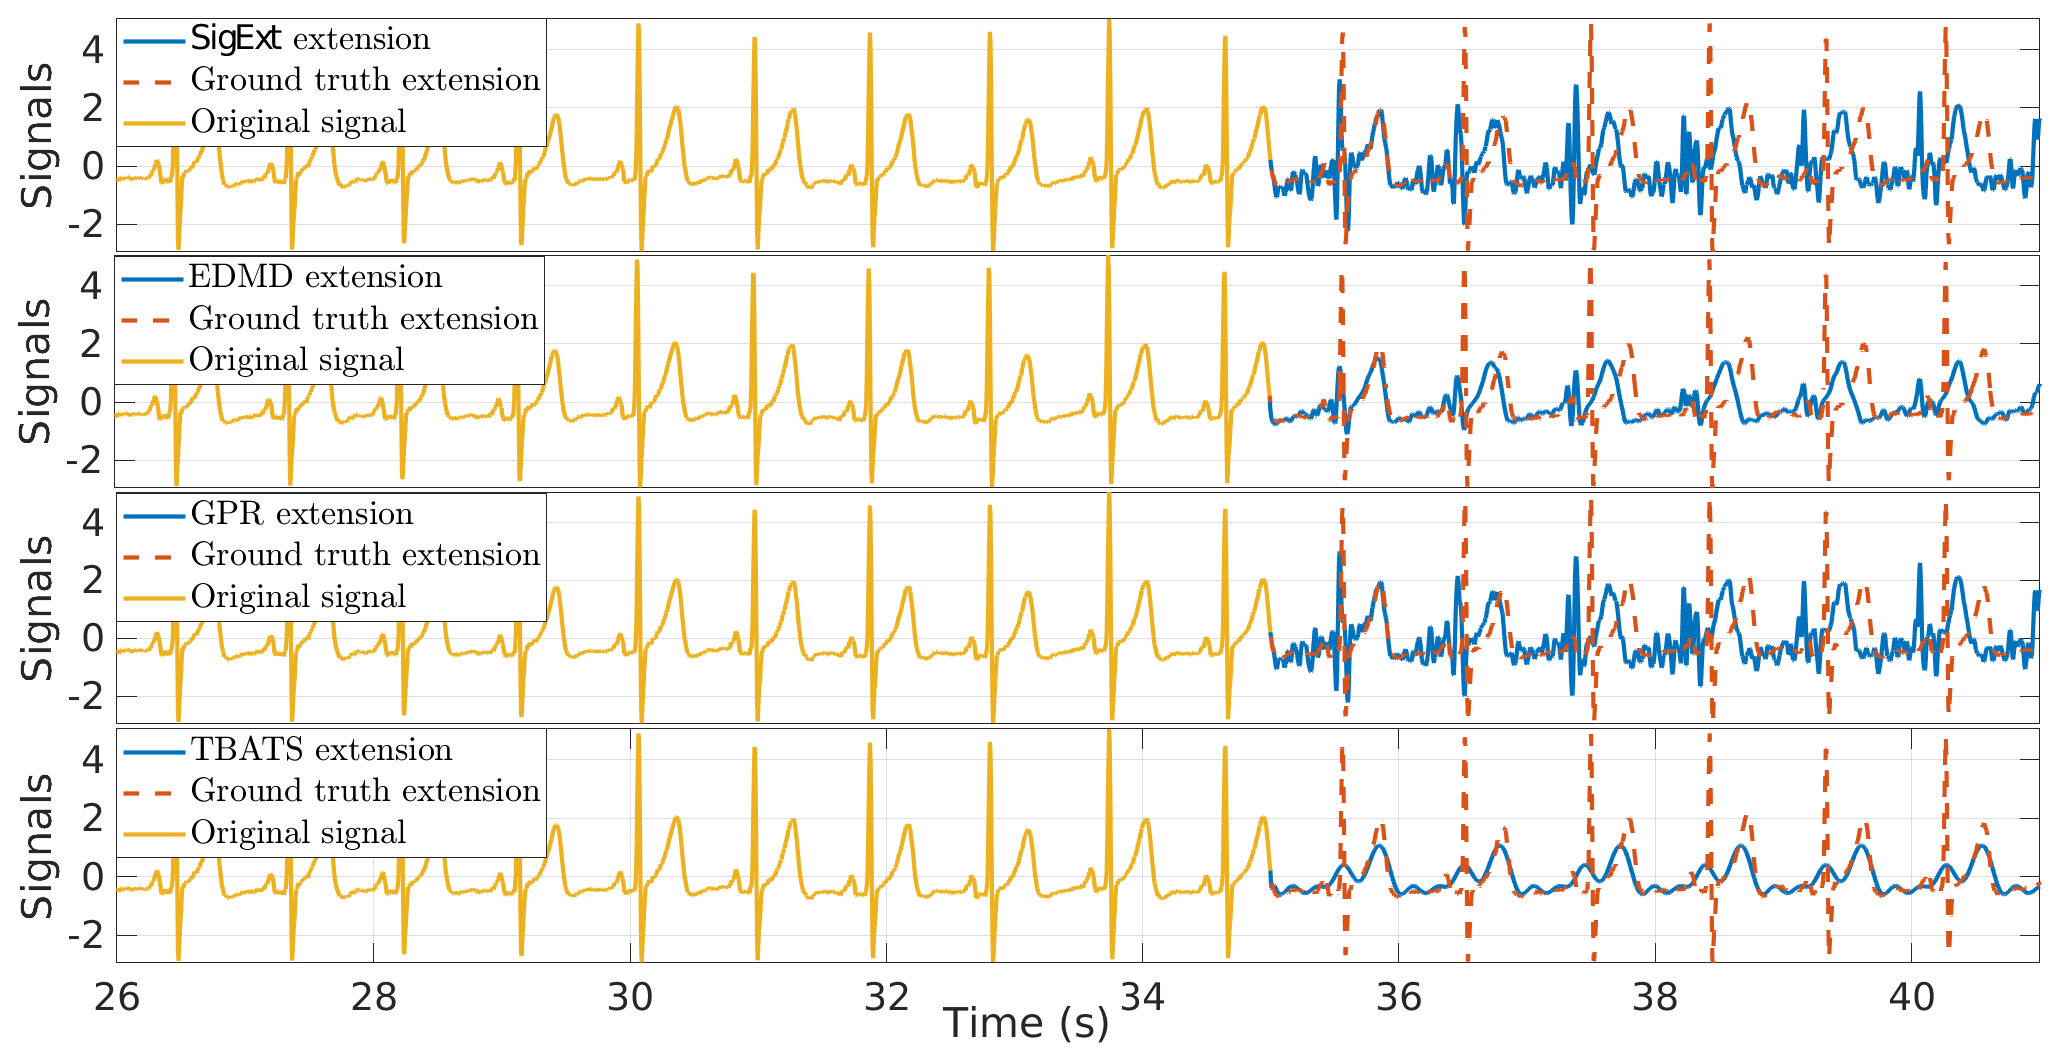
\includegraphics[width=\textwidth]{ECGforecast.eps}
\caption{Extended ECG (blue) obtained by the {\sf SigExt} forecasting (first panel), the EDMD forecasting (second panel), the GPR forecasting (third panel), and the TBATS forecasting (fourth panel), superimposed with the ground truth signal (dashed red).}
\label{fig:ecg}
\end{figure}

Table~\ref{tab:otd.ecg} contains the median performance index $D$ of the boundary-free TF representations, over the $N$ subsignals evaluated, according to the extension method. As a result of the fair quality of the forecasts, the reduction of boundary effects is less significant than for PPG signal. Nevertheles, the results show that {\sf BoundEffRed} has the same efficiency when the {\sf SigExt} extension, the EDMD extension or the GPR extension is chosen. Indeed, t-tests performed under the null hypothesis that the mean are equals, with a $5\%$ significance level, show no statistical significant difference between {\sf SigExt} and EDMD or GPR, regardless of the representation considered. This justifies the choice of {\sf SigExt} for real-time implementation.

\begin{table}
\centering
\caption{ECG: Performance of the Boundary-Free TF Representations According to the Extension Method}
\begin{tabular}{|c||c|c|c|c|}
  \hline
   \multirow{2}{40pt}{\centering Extension method} & \multicolumn{4}{c|}{Median performance index $D$} \\
   \cline{2-5}
      & STFT & SST & ConceFT & RS\\
   \hhline{|=#=|=|=|=|}
   {\sf SigExt} & $0.584$ & $0.630$ & $0.462$ & $0.642$ \\
   \hline
   Symmetric & $1.199$ & $1.354$ & $1.427$ & $0.943$ \\
   \hline
   EDMD & $0.538$ & $0.558$ & $0.496$ & $0.714$ \\
   \hline
   GPR & $0.639$ & $0.588$ & $0.485$ & $0.616$ \\
   \hline
\end{tabular}
\label{tab:otd.ecg}
\end{table}

%{\color{red}
%\section{Application to a Multicomponent Physiological Signal}
%}


\bibliographystyle{IEEEtran}
\bibliography{../AM041320}

\end{document}